\subsection{Development Methodology}
The CodingInfinity team will be using the \textbf{Agile Software Development methodology} during the course of the project. Agile Software Development is an umbrella term used to refer to the values and principles expressed in the Agile Manifesto.

In particular we find value in the following four points:
\begin{itemize}
	\item \textbf{Individuals and interactions} over processes and tools.
	\item \textbf{Working software} over comprehensive documentation.
	\item \textbf{Customer collaboration} over contract negotiation.
	\item \textbf{Responding to change} over following a plan.
\end{itemize}

Although we find value in the items on the right, we value the items on the left, emphasised in bold, even more.

The Agile principles themselves are derived from the following twelve principles:
\begin{itemize}
  \item Customer satisfaction by early and continuous delivery of valuable software
  \item Welcome changing requirements, even in late development
  \item Working software is delivered frequently (weeks rather than months)
  \item Close, daily cooperation between business people and developers
  \item Projects are built around motivated individuals, who should be trusted
  \item Face-to-face conversation is the best form of communication (co-location)
  \item Working software is the principal measure of progress
  \item Sustainable development, able to maintain a constant pace
  \item Continuous attention to technical excellence and good design
  \item Simplicity—the art of maximizing the amount of work not done—is essential
  \item Best architectures, requirements, and designs emerge from self-organizing teams
  \item Regularly, the team reflects on how to become more effective, and adjusts accordingly
\end{itemize}

Agile development seeks to provide opportunities to assess the changing functional and technical landscape while maintaining focus on rapid and continuous delivery of business value. This results in decreased overall risk associated with software development.

A core focus in Agile software development is to ensure that value is continuously derived through the development life cycle, which is achieved through a process of continuous planning and feedback. This process creates a feedback loop ensuring that the delivered software can be continuously aligned with the desired business needs and creates the opportunity for easy adoption to changing requirements throughout the process.

With continuous monitoring and measuring of the project status through continuous testing the client gains much more visibility into and around the actual progress of the project.

As a result of following an Agile Development approach the final deliverable software system will be able to much better address the business and customer needs than what would have produced with alternative methodologies.

\begin{figure}[t]
  \centering
  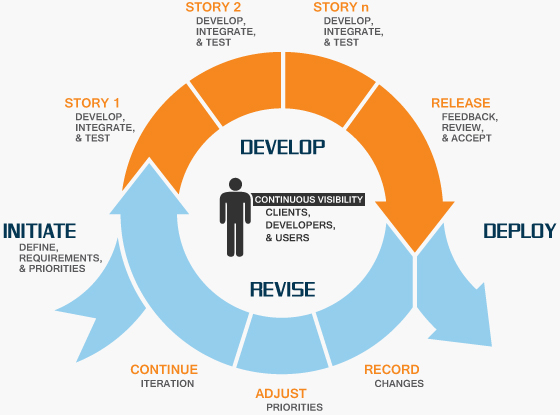
\includegraphics[scale=0.6]{agile.jpg}
  \caption{Agile Development Process}
\end{figure}


\subsection{Informing the Client}
\begin{itemize}
	\item Since the client is on site we will have weekly meetings where we will report on what has been done in the past week and discuss what will be done in the coming week. This is also in line with the Aglie development methodology that has been chosen.
	\item Email will be used if the team has questions for the client that can not wait until the next meeting.
	\item The client may request access to the developers scrum server and Slack communication if desired.
\end{itemize}

\subsection{Initial Ideas on Solving Some Technical Challenges}
\begin{itemize}
	\item Using a low level programming language such as C or C++ with assembly to gain access to the underlying hardware in order to be able to calculate the correct values for the benchmarking system.
	\item Use a REST based communication architecture to allow for integration with a web interface and mobile application.
	\item Utilizing git, DevOps with a Continuous Integration and Continuous Deployment to separate production and development code, while following an Agile methodology to continuously push new features to a live demo system.
	\item We will be making use of Docker with a REST based microservices architecture to allow for scalability, reliability and performance.
\end{itemize}

\subsection{Technologies We will Use}
\begin{itemize}
	\item Spring Framework \\
		We will be making extensive use of the Spring Framework which provides Dependency Injection, Aspect Oriented Programming, Spring Cloud to build distributed microservices and various other Spring projects.
	\item Spring Cloud with Netflix OSS \\
		Utilizing Spring Cloud with Netflix OSS components will allow one to build a very stable, scalable and reliable service which will be of great value to the wider open source community.
	\item JVM Language \\
		The backend management service will utilize a combination of a JVM language, like Java or Groovy, with the Spring Framework and Netflix OSS components.   A low level language such as C, C++ or assembly will be used to do the actual measurements.
	\item AngularJS \\
		For the frontend web interface AngularJS will be used to connect to the backend REST service to provide a user friendly interface to interact with the system. The web interface will expose both a user and administration section. The administration section will allow one to gain an overview and manage the software system deployment.
	\item Android \\
		The mobile application will be built and deployed for the Android operating system. The mobile application will allow users to view their aggreagted results from there mobile application. If time permits, the possibility of exporting data from a users Android device in real-time to the backend system will be explored.
	\end{itemize}

\subsection{What Will The Client Receive}
On completion of the development cycle the client will receive the following deliverables:
\begin{itemize}
	\item The functional application, which includes:
	\begin{itemize}
		\item The backend which will run the benchmarking tests and record the results
		\item A REST based web interface
		\item A REST based Android application
	\end{itemize}
	\item The source code for the functional application, unit and integration tests
	\item Associated build files
	\item The full specification documentation as required by the Agile Development methodology
	\item A user manual, however as one of the stated goals of the project is to develop a generic, easy to use benchmarking system that the user can use without training, this goal will need to be further discussed with the client.
\end{itemize}
